\documentclass[runningheads]{llncs}

\usepackage[T1]{fontenc}
\usepackage{graphicx}
\usepackage{amsmath,amssymb,amsfonts}
\usepackage{xcolor}
\usepackage{placeins}
\usepackage{url}
\usepackage{algorithm}
\usepackage{algpseudocode}
\usepackage{enumitem}
\renewcommand{\textfraction}{0.05}
\renewcommand{\topfraction}{0.95}
\renewcommand{\bottomfraction}{0.95}
\renewcommand{\floatpagefraction}{0.35}
\setcounter{totalnumber}{5}
\usepackage[font=small,skip=5pt]{caption}
\begin{document}

    \title{BloomSpan: Memory-Efficient Maximal Frequent Substring Mining for Large-Scale Text}

    \titlerunning{BloomSpan: Memory-Efficient Maximal Frequent Substring Mining}

    \author{Rauf Aliev\inst{1}\orcidID{0009-0006-2564-7742} \and
    Joeran Beel\inst{1}\orcidID{0000-0002-4537-5573}}

    \authorrunning{R. Aliev and J. Beel}

    \institute{University of Siegen, Siegen, Germany \\
    \email{r.aliev@gmail.com}, \email{joeran.beel@uni-siegen.de}}

    \maketitle

    \begin{abstract}
        BloomSpan is a memory-efficient algorithm for mining Maximal Contiguous Frequent Phrases (MCFPs) from large text corpora. MCFPs are strictly contiguous token sequences satisfying a minimum document-support threshold; unlike general Sequential Pattern Mining, no gaps are permitted. BloomSpan combines a Counting Bloom Filter for probabilistic frequency estimation with prioritized seed generation and depth-first expansion directly on the corpus, avoiding recursive projected databases. Seed generation is provably free of false negatives; output equivalence with exact baselines is confirmed on all Gutenberg-8k subsets where any baseline completes. On the \texttt{Gutenberg-BookCorpus-Cleaned} corpus (up to 3.07\,B tokens), BloomSpan achieves 11-15x faster wall-clock execution than FHK with up to 2x lower peak memory.
        \keywords{Frequent substring mining \and Maximal contiguous phrases \and Suffix array \and Counting Bloom Filter \and Large-scale text corpora}
    \end{abstract}

    \section{Introduction}

    The identification of frequent patterns within large sequences is a cornerstone problem in data mining. General Sequential Pattern Mining (SPM) algorithms such as GSP~\cite{agrawal1995mining} and PrefixSpan~\cite{pei2001prefixspan} allow arbitrary gaps between elements and treat each element as a set (itemset). While mathematically powerful, this generality is a liability in domains such as document template extraction, plagiarism detection, and phrase mining, where patterns are single tokens forming rigid, unbroken structures. Introducing gaps into such searches leads to a \emph{combinatorial explosion} of meaningless candidates: given a sequence $\langle A, B, C \rangle$, an SPM miner considers the pattern present even when elements appear as $A \dots \text{gap} \dots B \dots \text{gap} \dots C$, generating orders of magnitude more candidates than the contiguous case requires. The Maximal Contiguous Frequent Phrase (MCFP) mining problem~\cite{fischer2006fast} captures the constrained setting where no gap is allowed and each element is a single token.

    Practitioners navigating this problem face a dichotomy of extremes. \emph{Stringology-native suffix-array miners} build on decades of index engineering starting with Manber and Myers' suffix array~\cite{manber1993suffix}, Kasai et al.'s linear-time LCP construction~\cite{kasai2001linear}, and the enhanced suffix array framework of Abouelhoda, Kurtz, and Ohlebusch~\cite{abouelhoda2004replacing}; practical deployments further rely on Nong--Zhang--Chan's SA-IS suffix array construction~\cite{nong2011saiis} and, for compressed settings, on the FM-index and related self-indexes surveyed by Navarro and M\"akinen~\cite{navarro2007compressed}. Specifically for substring mining, the Fischer--Heun--Kramer algorithm (FHK)~\cite{fischer2005icdm,fischer2009dami}, the Deferred Frequency Index (DFI~\cite{weese2008dfi}), and related work~\cite{kugel2008space,dhaliwal2012practical,fischer2008space} solve MCFP in asymptotically optimal time but carry constant factors that become significant on large natural-language alphabets and permissive operating points. Recent work at SPIRE~2024 continues to refine this line, including online~\cite{guo2024netfreq} and faster offline~\cite{ohlebusch2024chinese} computation of closely related net-frequency queries. BloomSpan complements this line by moving orthogonally: it targets a document-frequency constraint on a bounded-memory probabilistic substrate rather than an exact index, trading worst-case guarantees for empirical memory savings on large natural-language corpora. \emph{Gap-aware sequence miners} (BIDE+~\cite{wang2004bide}, VMSP~\cite{fournier2014vmsp}) solve a strictly more general problem and manage a much larger search space, incurring severe memory pressure when restricted to contiguous extensions.

    We present \emph{BloomSpan}, which occupies a distinct operating point between these families: a Counting Bloom Filter bypasses explicit candidate generation, while a depth-first expansion with a global occupancy bitmask bounds memory to $O(W + M)$ in the input size. Our main contributions are:  (1) an algorithm whose runtime decomposes into an input-linear pre-processing component and a data-dependent expansion component, scaling near-linearly per token on a 3 billion-token natural-language corpus at strict thresholds ($\sigma \geq 20$); (2) a probabilistic seed-filtering mechanism that provably produces no false negatives.


    \section{Problem Formalization}\label{sec:problem-formalization}

    Let $\Sigma$ be a finite token alphabet. A document $d_i = (t_1,\dots,t_n)$ is an ordered token sequence. Given corpus $\mathcal{C} = \{d_1,\dots,d_m\}$ and support threshold $\sigma$, the task is to extract all MCFPs.

    \begin{itemize}[noitemsep, topsep=0pt]
        \item \textbf{Phrase ($P$):} A \textbf{strictly contiguous} subsequence $(t_i, t_{i+1}, \dots, t_{i+k-1})$.
        \item \textbf{Support ($df$):} $df(P) = |\{d \in \mathcal{C} : P \text{ appears in } d\}|$.
        \item \textbf{Seed ($S$):} A frequent $n$-gram ($df(S) \ge \sigma$) serving as an expansion anchor.
        \item \textbf{MCFP:} A phrase $P$ with $df(P) \ge \sigma$ such that no strict super-phrase $P'$ containing $P$ satisfies $df(P') \ge \sigma$.
    \end{itemize}


    \section{Proposed Algorithm: BloomSpan}

    \begin{algorithm}[t]
\caption{BloomSpan (top-level)}
\label{alg:bloomspan}
\begin{algorithmic}[1]
    \Require Corpus $\mathcal{C}$, support threshold $\sigma$, seed length $n$, minimum phrase length $\ell_{\min}$
    \Ensure Set $\mathcal{M}$ of MCFPs
    \State $\mathit{df}_1 \gets$ exact 1-gram document frequencies over $\mathcal{C}$
    \State $\hat{c} \gets$ CBF populated with all length-$n$ windows of $\mathcal{C}$
    \State $\mathcal{S} \gets \{ S : \hat{c}(S) \geq \sigma \wedge \min_{t \in S} \mathit{df}_1(t) \geq \sigma \}$ \Comment{seed candidates}
    \State $\mathcal{S}' \gets$ merge $\mathcal{S}$ by exact $df$, keep those with $df \geq \sigma$
    \State sort $\mathcal{S}'$ by $\Psi(S) = |S| \cdot df(S)$ desc., then length desc., then lex.
    \State $\mathit{occupied} \gets$ all-zeros bitmask over $\sum_d |d|$ positions
    \State $\mathcal{M} \gets \emptyset$
    \For{each candidate $S \in \mathcal{S}'$ in order}
        \If{all occurrences of $S$ lie in $\mathit{occupied}$ positions} \textbf{continue} \EndIf
        \State DFS-Expand($S$, $\mathit{occupied}$, $\mathcal{M}$) \Comment{Algorithm 2}
    \EndFor
    \State \Return $\mathcal{M}$
\end{algorithmic}
    \end{algorithm}

    BloomSpan transitions from pattern-growth projection trees to a prioritized Depth-First Search (DFS) combined with probabilistic filtering. It operates in four phases.

    \subsection{Phase 1: Database Loading and Probabilistic Frequency Estimation}
    The corpus is loaded and exact 1-gram document frequencies $df(t)$ are computed. A Counting Bloom Filter (CBF)~\cite{fan2000summary} (up to 512\,MB) is populated with all $n$-grams ($n \ge 2$) via a linear pass, providing a space-efficient frequency sketch akin to the Count-Min Sketch~\cite{cormode2005improved}.

    \begin{figure}[!t]
        \centering
        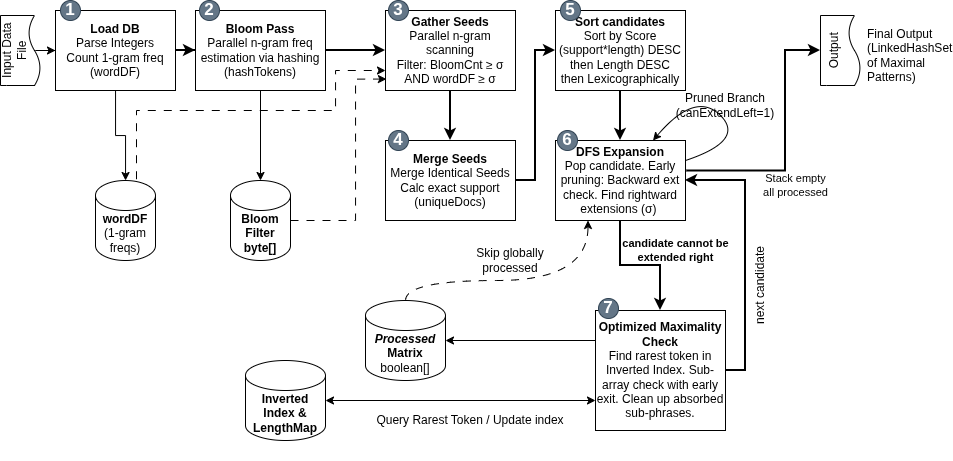
\includegraphics[width=\textwidth]{algorithm.png}
        \caption{BloomSpan pipeline overview.}
        \label{fig:pipeline}
    \end{figure}

    \subsection{Phase 2: Seed Candidate Generation and Prioritization}
    A parallel corpus scan identifies $n$-gram seeds. A candidate is pruned if (a)~its CBF estimate is below $\sigma$, or (b)~any constituent 1-gram has $df < \sigma$. The CBF maintains an estimate $\hat{c}(S)$ of the total corpus occurrence count $c(S) = \sum_{d \in \mathcal{C}} \#\{i : d[i..i+n-1] = S\}$. Hash collisions can only over-estimate this count, so $\hat{c}(S) \geq c(S)$. Since each document containing $S$ contributes at least one occurrence to $c(S)$, we have $c(S) \geq df(S)$ trivially. Composing both inequalities, $\hat{c}(S) \geq df(S)$, so any $S$ with true $df(S) \geq \sigma$ passes the filter $\hat{c}(S) \geq \sigma$. By the anti-monotonicity of document frequency, every MCFP of length $\ell \geq n$ contains at least one length-$n$ contiguous sub-sequence $S$ with $df(S) \geq \sigma$; hence every truly frequent longer phrase remains reachable from a surviving seed. Together these two properties guarantee no truly frequent pattern is pruned at this stage. (We track $c(\cdot)$ rather than $df(\cdot)$ to avoid the per-document reset cost on a CBF; the inequality $c \geq df$ is sufficient for the guarantee, and exact $df$ values are recomputed in $O(\text{occ})$ time during seed merging in Phase 2.). The CBF filter is loose with respect to $df$ — a bigram occurring 20 times within a single document passes — so absolute pruning ratios depend on the corpus topology. On Realistic Dataset~2 at $\sigma = 20$, $n = 2$ (Section~\ref{sec:results-large}), the combined CBF-and-1-gram filter eliminates 98\% of candidate $n$-grams; we report per-corpus pruning ratios in Section~\ref{sec:results-large}. Valid seeds are assigned a coverage score $\Psi(P) = |P| \times df(P)$ and globally sorted by it, with ties broken first by descending length and then lexicographically, so that larger, more frequent ``backbone'' patterns are processed first.

    \subsection{Phase 3: DFS Expansion and Early Pruning}
    Expansion is performed directly on the original corpus using a stack, avoiding projected databases. Before right-extension, an \emph{Early Pruning} step checks whether all occurrences of a candidate share the same preceding token; if so, the candidate is inherently non-maximal and is immediately pruned.

    \subsection{Phase 4: Maximality Check and Redundancy Control}
    An \emph{Inverted Index} keyed on each pattern's rarest token reduces the maximality check from an $O(P \times l_p)$ scan to an $O(p_\text{rare} \times l_p)$ lookup ($p_\text{rare} \ll P$). If a candidate is confirmed maximal, BloomSpan also absorbs and removes any previously discovered sub-phrases now subsumed by the longer pattern. A global \emph{occupancy bitmask} flags all token positions belonging to confirmed maximal patterns; any subsequent candidate whose occurrences lie entirely within already-flagged positions is skipped before expansion.

    \subsection{Complexity}
    Let $W$ = total tokens, $M$ = CBF size, $C$ = valid seed occurrences, $P$ = maximal patterns found.

    \textbf{Space:} $O(W + M + C + P)$. The corpus and bitmask each require $O(W)$; the CBF uses exactly $M$ bytes; seed and index structures require $O(C + P \cdot l_p)$.

    \textbf{Time:} Let $W$ = total tokens, $n$ = seed length (a constant; $n = 2$ throughout), $C$ = surviving seed occurrences after Phase~2, and $P$ = MCFPs in the output. Phase~1 (CBF population and 1-gram counting) takes $\Theta(W)$. Phase~2 (seed gathering, parallel scan and sort) takes $\Theta(W + C \log C)$. Phase~3 (DFS expansion) is data-dependent: each expansion step over a candidate with $s$ occurrences takes $O(s)$ for the early-pruning check and the next-token grouping, and the inverted-index maximality check costs $O(p_\text{rare} \cdot l_p \cdot l_\text{super})$ per candidate, where $p_\text{rare}$ is the number of MCFPs containing the candidate's rarest token. We do not establish a worst-case bound on Phase~3; instead, Section~\ref{sec:results-large} reports approximately constant per-token mining cost (0.021–0.027\,$\mu$s/token, log-log slope 0.98) across a 28$\times$ range of input sizes at $\sigma = 20$, with a transition to super-linear scaling once the MCFP set itself grows large.

    \section{Experimental Evaluation}

    \subsection{Setup}
    All algorithms are evaluated as JVM-based implementations on the same machine (Ultra~9, 64\,GB RAM, OpenJDK~21,\texttt{-Xmx40g}); evaluating BloomSpan, FHK, and DFI within a single language stack ensures that reported speedups reflect algorithmic differences rather than runtime artifacts. SPMF baselines (GST/SA+LCP, VMSP, BIDE+) use the SPMF framework~\cite{fournierviger2016spmf} (v2.65); FHK and DFI are in-house Java implementations. Reported times are wall-clock from algorithm invocation to termination, measured identically by a common benchmark runner; includes corpus parsing and, for FHK/DFI, suffix and LCP array construction, excludes one-time conversion to the SPMF int-encoded format (before the timed region, identical across algorithms). Each (algorithm, $N$) configuration was executed for 6 runs; the 1st is discarded as JVM warm-up, and medians with inter-quartile ranges (IQR) over the remaining 5 are reported. We use medians because occasional GC pauses introduce positive skew; across all BloomSpan runs the relative time IQR stayed below 5\% of the median. Source code: \url{https://github.com/raliev/bloomspan}.

    \subsection{Baselines}
    \begin{enumerate}
        \item \textbf{FHK} --- in-house Java implementation of Fischer--Heun--Kramer~\cite{fischer2006fast,fischer2009dami}: SA-IS suffix array~\cite{nong2011saiis}, Kasai LCP array~\cite{kasai2001linear}, stack-based bottom-up LCP-interval traversal.
        \item \textbf{DFI} --- in-house Java implementation of the Deferred Frequency Index~\cite{weese2008dfi}: same SA-IS + Kasai preprocessing, top-down DFS with early subtree pruning and an $O(n \log n)$ RMQ sparse table.
        \item \textbf{GST/SA+LCP} --- suffix-array baseline from SPMF.
        \item \textbf{VMSP} --- maximal sequential pattern miner from SPMF~\cite{fournier2014vmsp}; included as a sanity check.
        \item \textbf{BIDE+ (Contiguous Maximal)} --- maximal sequence miner~\cite{wang2004bide} restricted to contiguous extensions.
    \end{enumerate}

    \subsection{Datasets}

    We evaluate on two synthetic and two realistic datasets covering a wide range of corpus sizes and pattern topologies.

    \begin{itemize}[noitemsep, topsep=0pt]
        \item \textbf{Synthetic Dataset 1 (Sparse Injections).} $N$ documents of 5000 unique synthetic words each, with three short fixed sentences injected into a small random subset of documents ($\sigma = 3$, min.\ phrase length 3). Sizes: $N = 100$--$30{,}000$.

        \item \textbf{Synthetic Dataset 2 (Dense Nested Overlaps).} 300 heavily overlapping sentences of incrementally decreasing length injected into a unique-word background ($N = 15{,}000$). Designed as a worst-case topology for BloomSpan's redundancy control.

        \item \textbf{Realistic Dataset 1 (Gutenberg-8k).} First $N$ files of \texttt{Fhrozen/gutenberg8k}~\cite{gutenberg8k} (8544 books, 535\,M tokens). Subsets characterised in Table~\ref{tab:gut_subsets}. Parameters: $\sigma = 10$, min.\ phrase length 5.

        \item \textbf{Realistic Dataset 2 (Gutenberg-BookCorpus-Cleaned).} First $N$ files of the 66{,}871-book Gutenberg-BookCorpus-Cleaned release~\cite{gutenbergcleaned} ($N$ up to 50{,}000, $\approx 3.07$\,B tokens). Parameters: $\sigma = 20$, min.\ phrase length 10. SPMF-based baselines exhaust the heap at $N = 1{,}000$ and are excluded.
    \end{itemize}

    \begin{table}[!tbp]
        \caption{Characterisation of Gutenberg-8k subsets. TTR = type/token ratio.}
        \begin{center}
            \resizebox{\textwidth}{!}{%
                \begin{tabular}{|c|r|r|r|r|r|r|r|}
                    \hline
                    \textbf{N} & \textbf{Size} & \textbf{Total tokens} & \textbf{Vocabulary} & \multicolumn{3}{|c|}{\textbf{Tokens / document}} & \textbf{TTR} \\
                    \cline{5-7}
                    & & & & \textbf{median} & \textbf{mean} & \textbf{max} & \\
                    \hline
                    100   & 21.2\,MB   & 3{,}913{,}260   & 263{,}784    & 18{,}376 & 39{,}132 & 162{,}961   & 0.0674 \\
                    250   & 72.0\,MB   & 13{,}272{,}683  & 591{,}817    & 38{,}618 & 53{,}090 & 259{,}595   & 0.0446 \\
                    500   & 156.1\,MB  & 28{,}438{,}195  & 1{,}022{,}479 & 38{,}445 & 56{,}876 & 467{,}524   & 0.0360 \\
                    1{,}000 & 324.1\,MB  & 58{,}853{,}177  & 1{,}900{,}504 & 42{,}945 & 58{,}853 & 763{,}654   & 0.0323 \\
                    3{,}000 & 1{,}015.1\,MB & 183{,}409{,}628 & 4{,}616{,}291 & 46{,}030 & 61{,}136 & 763{,}654   & 0.0252 \\
                    5{,}000 & 1.7\,GB    & 305{,}326{,}775 & 6{,}536{,}695 & 45{,}412 & 61{,}065 & 832{,}335   & 0.0214 \\
                    8{,}544 & 2.9\,GB    & 535{,}259{,}155 & 9{,}113{,}577 & 44{,}733 & 62{,}647 & 1{,}662{,}371 & 0.0170 \\
                    \hline
                \end{tabular}%
            }
            \label{tab:gut_subsets}
        \end{center}
    \end{table}

    \subsection{Results: Synthetic Dataset 1}

    Figure~\ref{fig:synth1} and Table~\ref{tab:synth1} show results for Synthetic Dataset~1.
    All stringology-native miners (FHK, DFI, BloomSpan) scale approximately linearly in time and memory up to $N = 10{,}000$.
    However, a performance crossover occurs at $N = 12{,}000$ ($0.6 \times 10^8$ tokens).
    Beyond this point, FHK becomes the most efficient algorithm in both dimensions.
    At $N = 30{,}000$, FHK completes in 15.3\,s using 38.9\,GB, whereas BloomSpan requires 38.2\,s and reaches the heap limit at 40.3\,GB.
    This shifts the previous observation: while BloomSpan is highly competitive on smaller synthetic sets, FHK's LCP-interval traversal proves more robust for the flat frequency distribution of unique synthetic background words at large scales. However, this changes for the realistic dataset.

    \begin{figure}[!tbp]
        \begin{minipage}{0.49\textwidth}
            \centering
            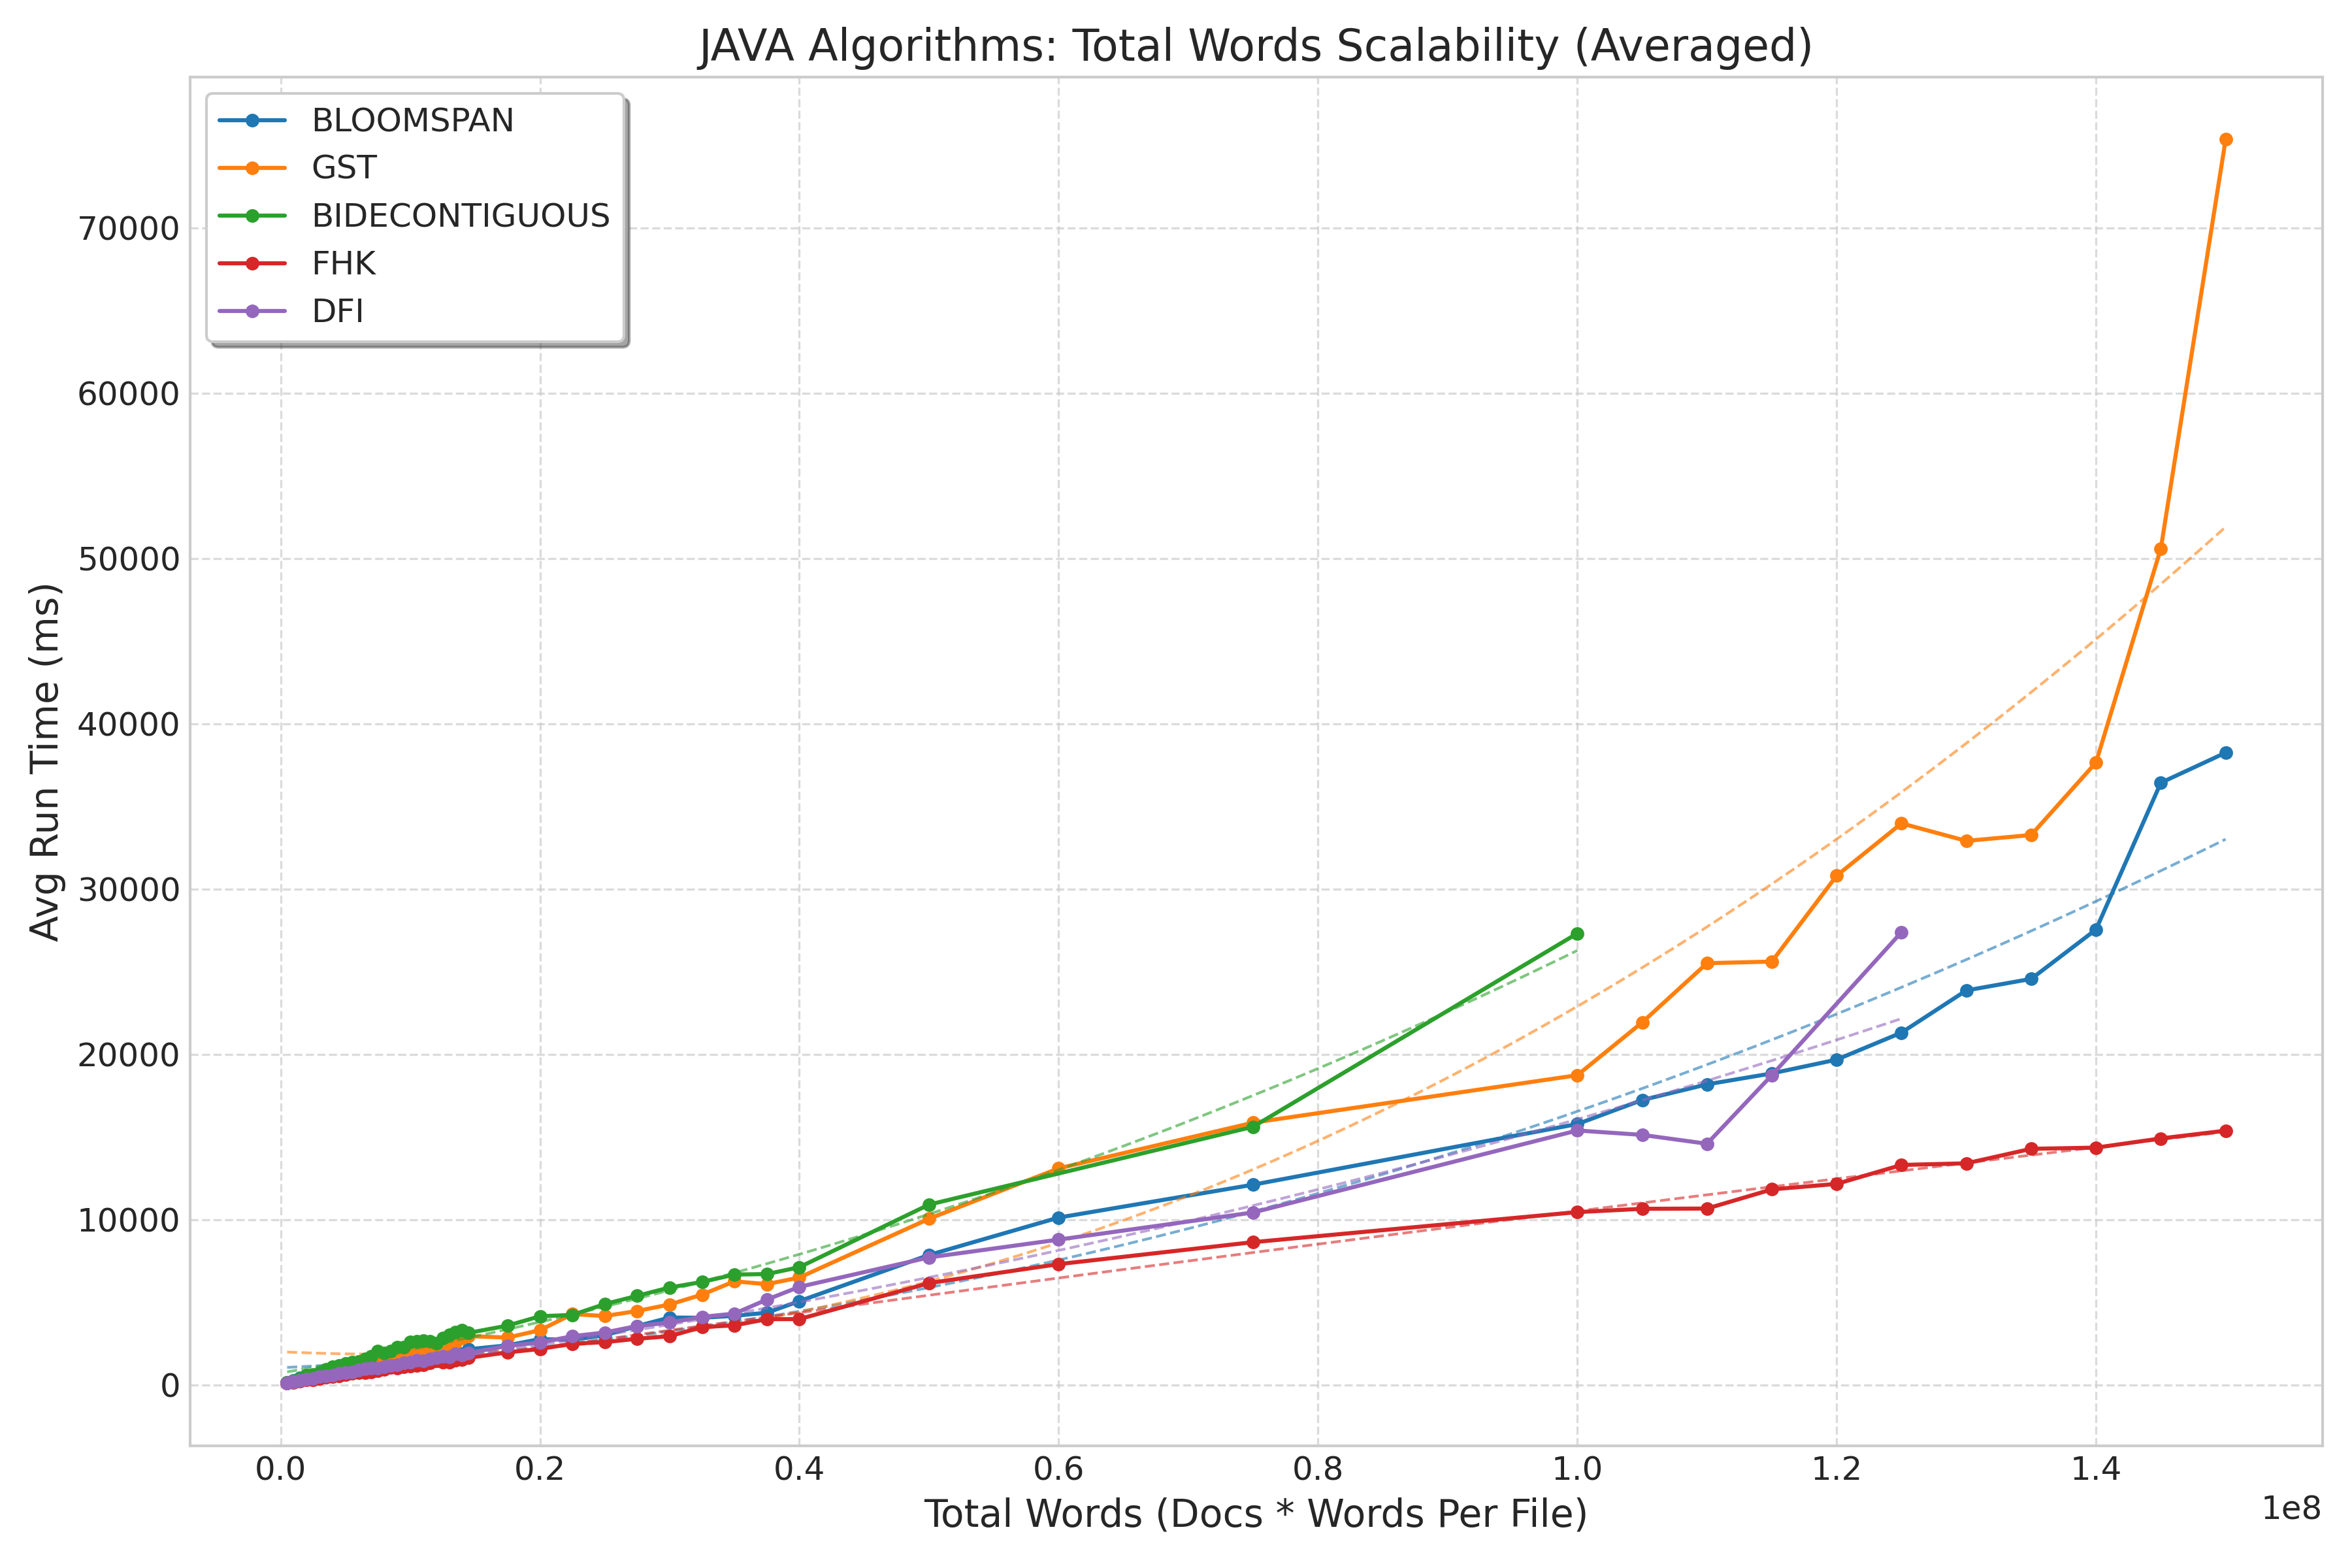
\includegraphics[width=\linewidth]{synthetic_time.png}
        \end{minipage}
        \hfill
        \begin{minipage}{0.49\textwidth}
            \centering
            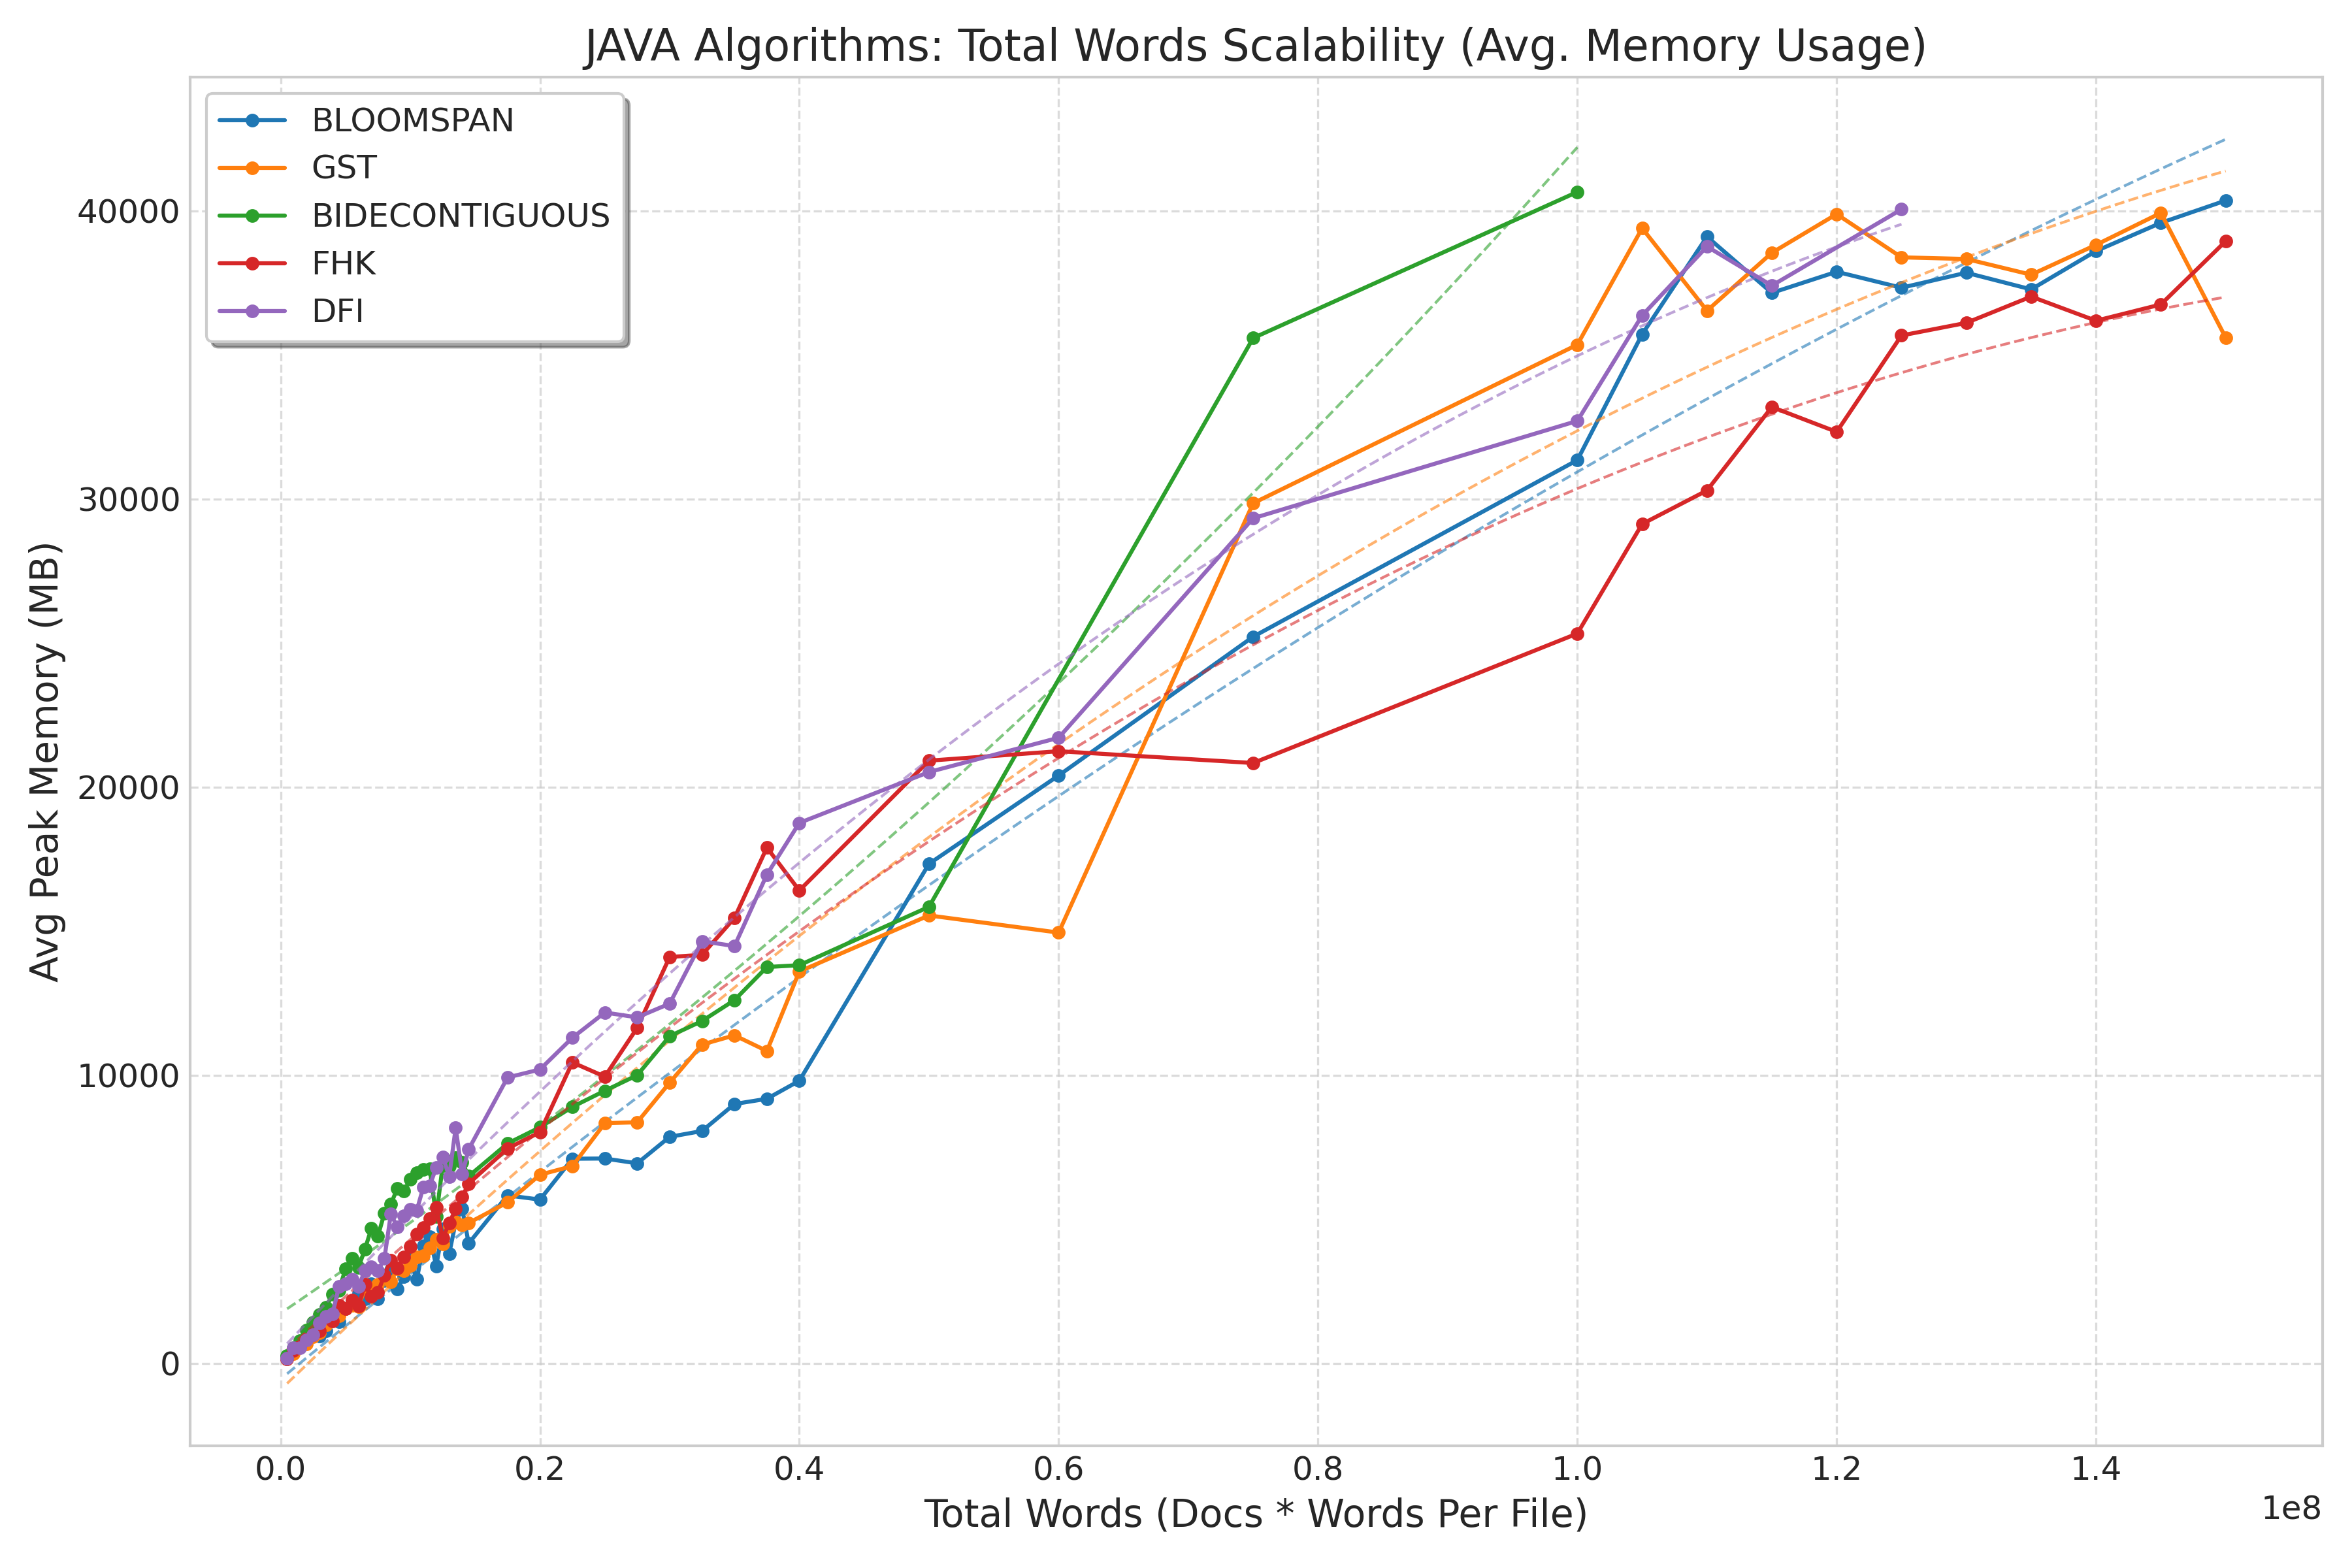
\includegraphics[width=\linewidth]{synthetic_memory.png}
        \end{minipage}
        \caption{Execution time (L) and peak memory (R) on Synthetic Dataset~1..}
        \label{fig:synth1}
    \end{figure}

    \begin{table}[!tbp]
        \caption{Performance on Synthetic Dataset 1 (5000 w/d). Time in ms; Mem in MB.}
        \begin{center}
            \resizebox{\textwidth}{!}{%
                \begin{tabular}{|c|cc|cc|cc|cc|}
                    \hline
                    \textbf{N (Docs)} & \multicolumn{2}{c|}{\textbf{BloomSpan}} & \multicolumn{2}{c|}{\textbf{FHK}} & \multicolumn{2}{c|}{\textbf{DFI}} & \multicolumn{2}{c|}{\textbf{GST/SA+LCP}} \\
                    \cline{2-9}
                    & \textbf{Time} & \textbf{Mem} & \textbf{Time} & \textbf{Mem} & \textbf{Time} & \textbf{Mem} & \textbf{Time} & \textbf{Mem} \\
                    \hline
                    1{,}000  & 1{,}047  & 1{,}893  & 625    & 1{,}908  & 713    & 2{,}773  & 931    & 1{,}903  \\
                    10{,}000 & 7{,}852  & 17{,}339 & 6{,}151  & 20{,}920 & 7{,}704  & 20{,}525 & 10{,}041 & 15{,}548 \\
                    12{,}000 & 10{,}115 & 20{,}405 & 7{,}299  & 21{,}249 & 8{,}782  & 21{,}716 & 13{,}091 & 14{,}953 \\
                    20{,}000 & 15{,}772 & 31{,}351 & 10{,}446 & 25{,}332 & 15{,}384 & 32{,}711 & 18{,}727 & 35{,}356 \\
                    30{,}000 & 38{,}240 & 40{,}360 & 15{,}373 & 38{,}949 & OOM      & OOM      & 75{,}348 & 35{,}603 \\
                    \hline
                \end{tabular}%
            }
            \label{tab:synth1}
        \end{center}
    \end{table}

    \begin{table}[!tbp]
        \caption{Performance on Synthetic Dataset 2 at $N = 15{,}000$ (84\,M tokens). Medians with IQR over six runs. Time in ms; memory in MB.}
        \begin{center}
            \begin{tabular}{|l|c|c|}
                \hline
                \textbf{Algorithm} & \textbf{Time (ms)} & \textbf{Memory (MB)} \\
                \hline
                FHK                       & 10{,}461 (401)   & 23{,}166 (587)   \\
                BloomSpan                 & 12{,}589 (2{,}337) & 26{,}809 (2{,}942) \\
                DFI                       & 14{,}861 (280)   & 32{,}903 (971)   \\
                BIDE+ (Contig.\ Maximal) & 16{,}765 (318)   & 36{,}965 (866)   \\
                \hline
            \end{tabular}
            \label{tab:synth2}
        \end{center}
    \end{table}

    \begin{figure}[!tbp]
        \begin{minipage}{0.49\textwidth}
            \centering
            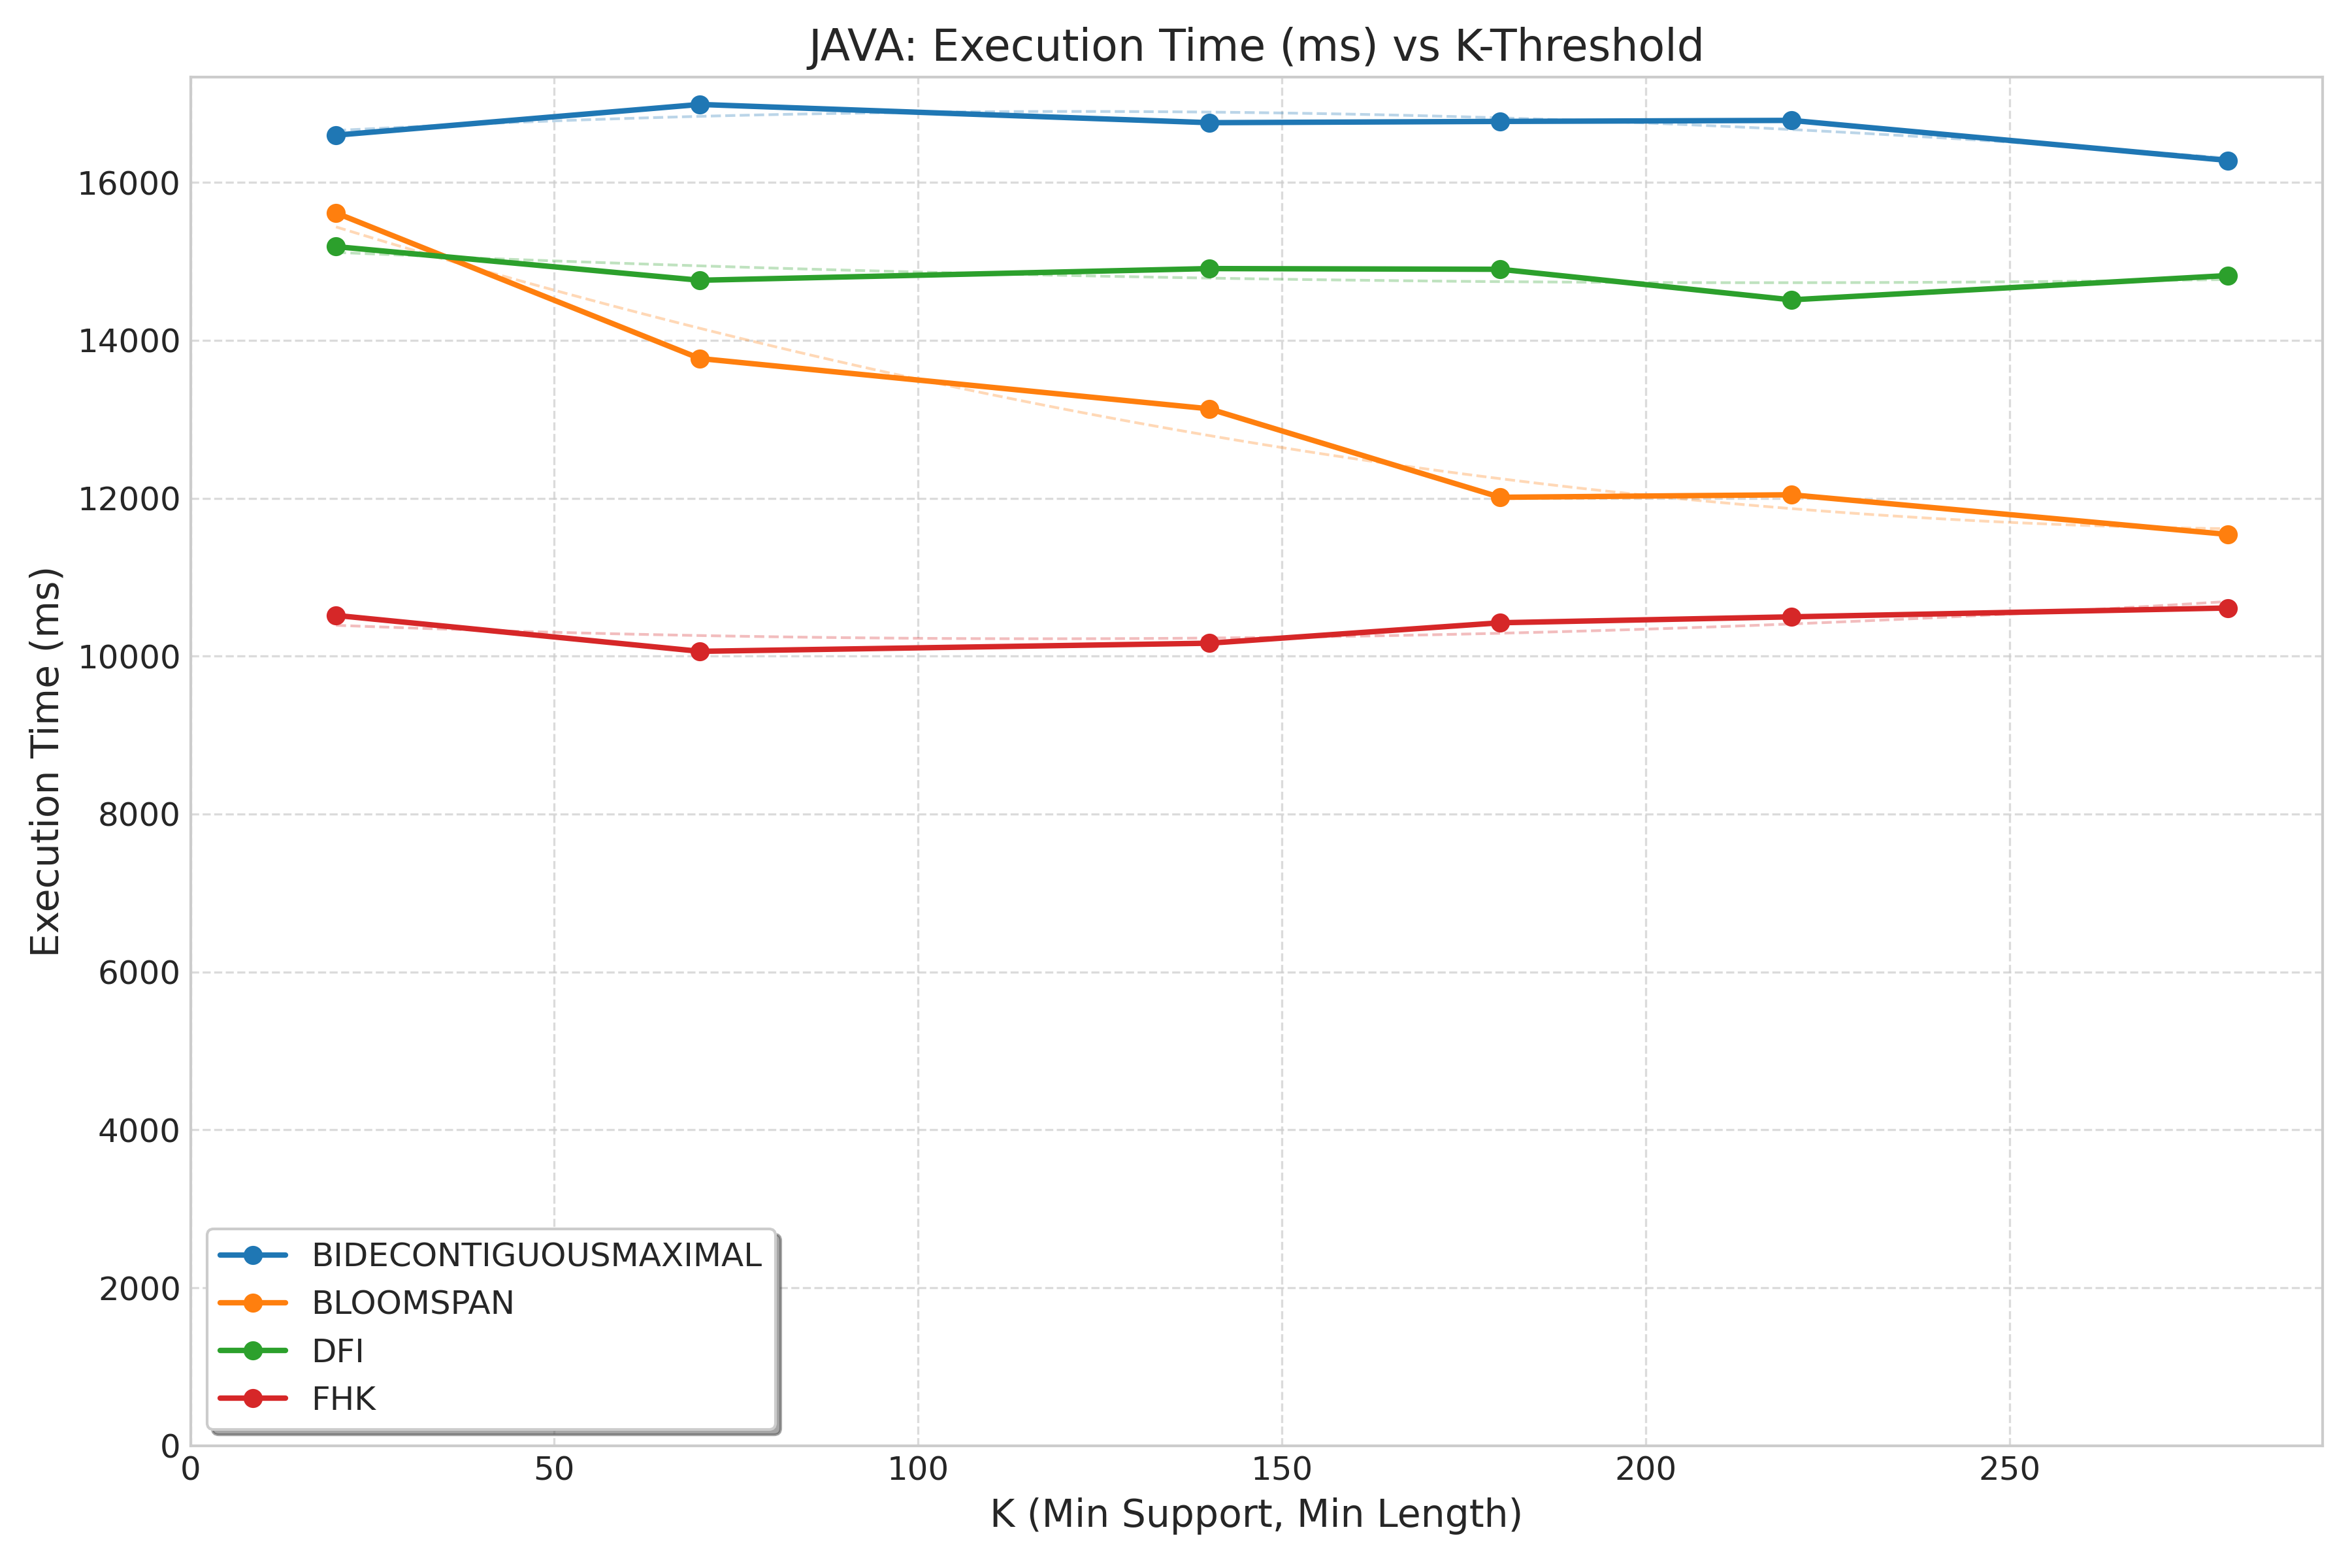
\includegraphics[width=\linewidth]{java_time_vs_k.png}
        \end{minipage}
        \hfill
        \begin{minipage}{0.49\textwidth}
            \centering
            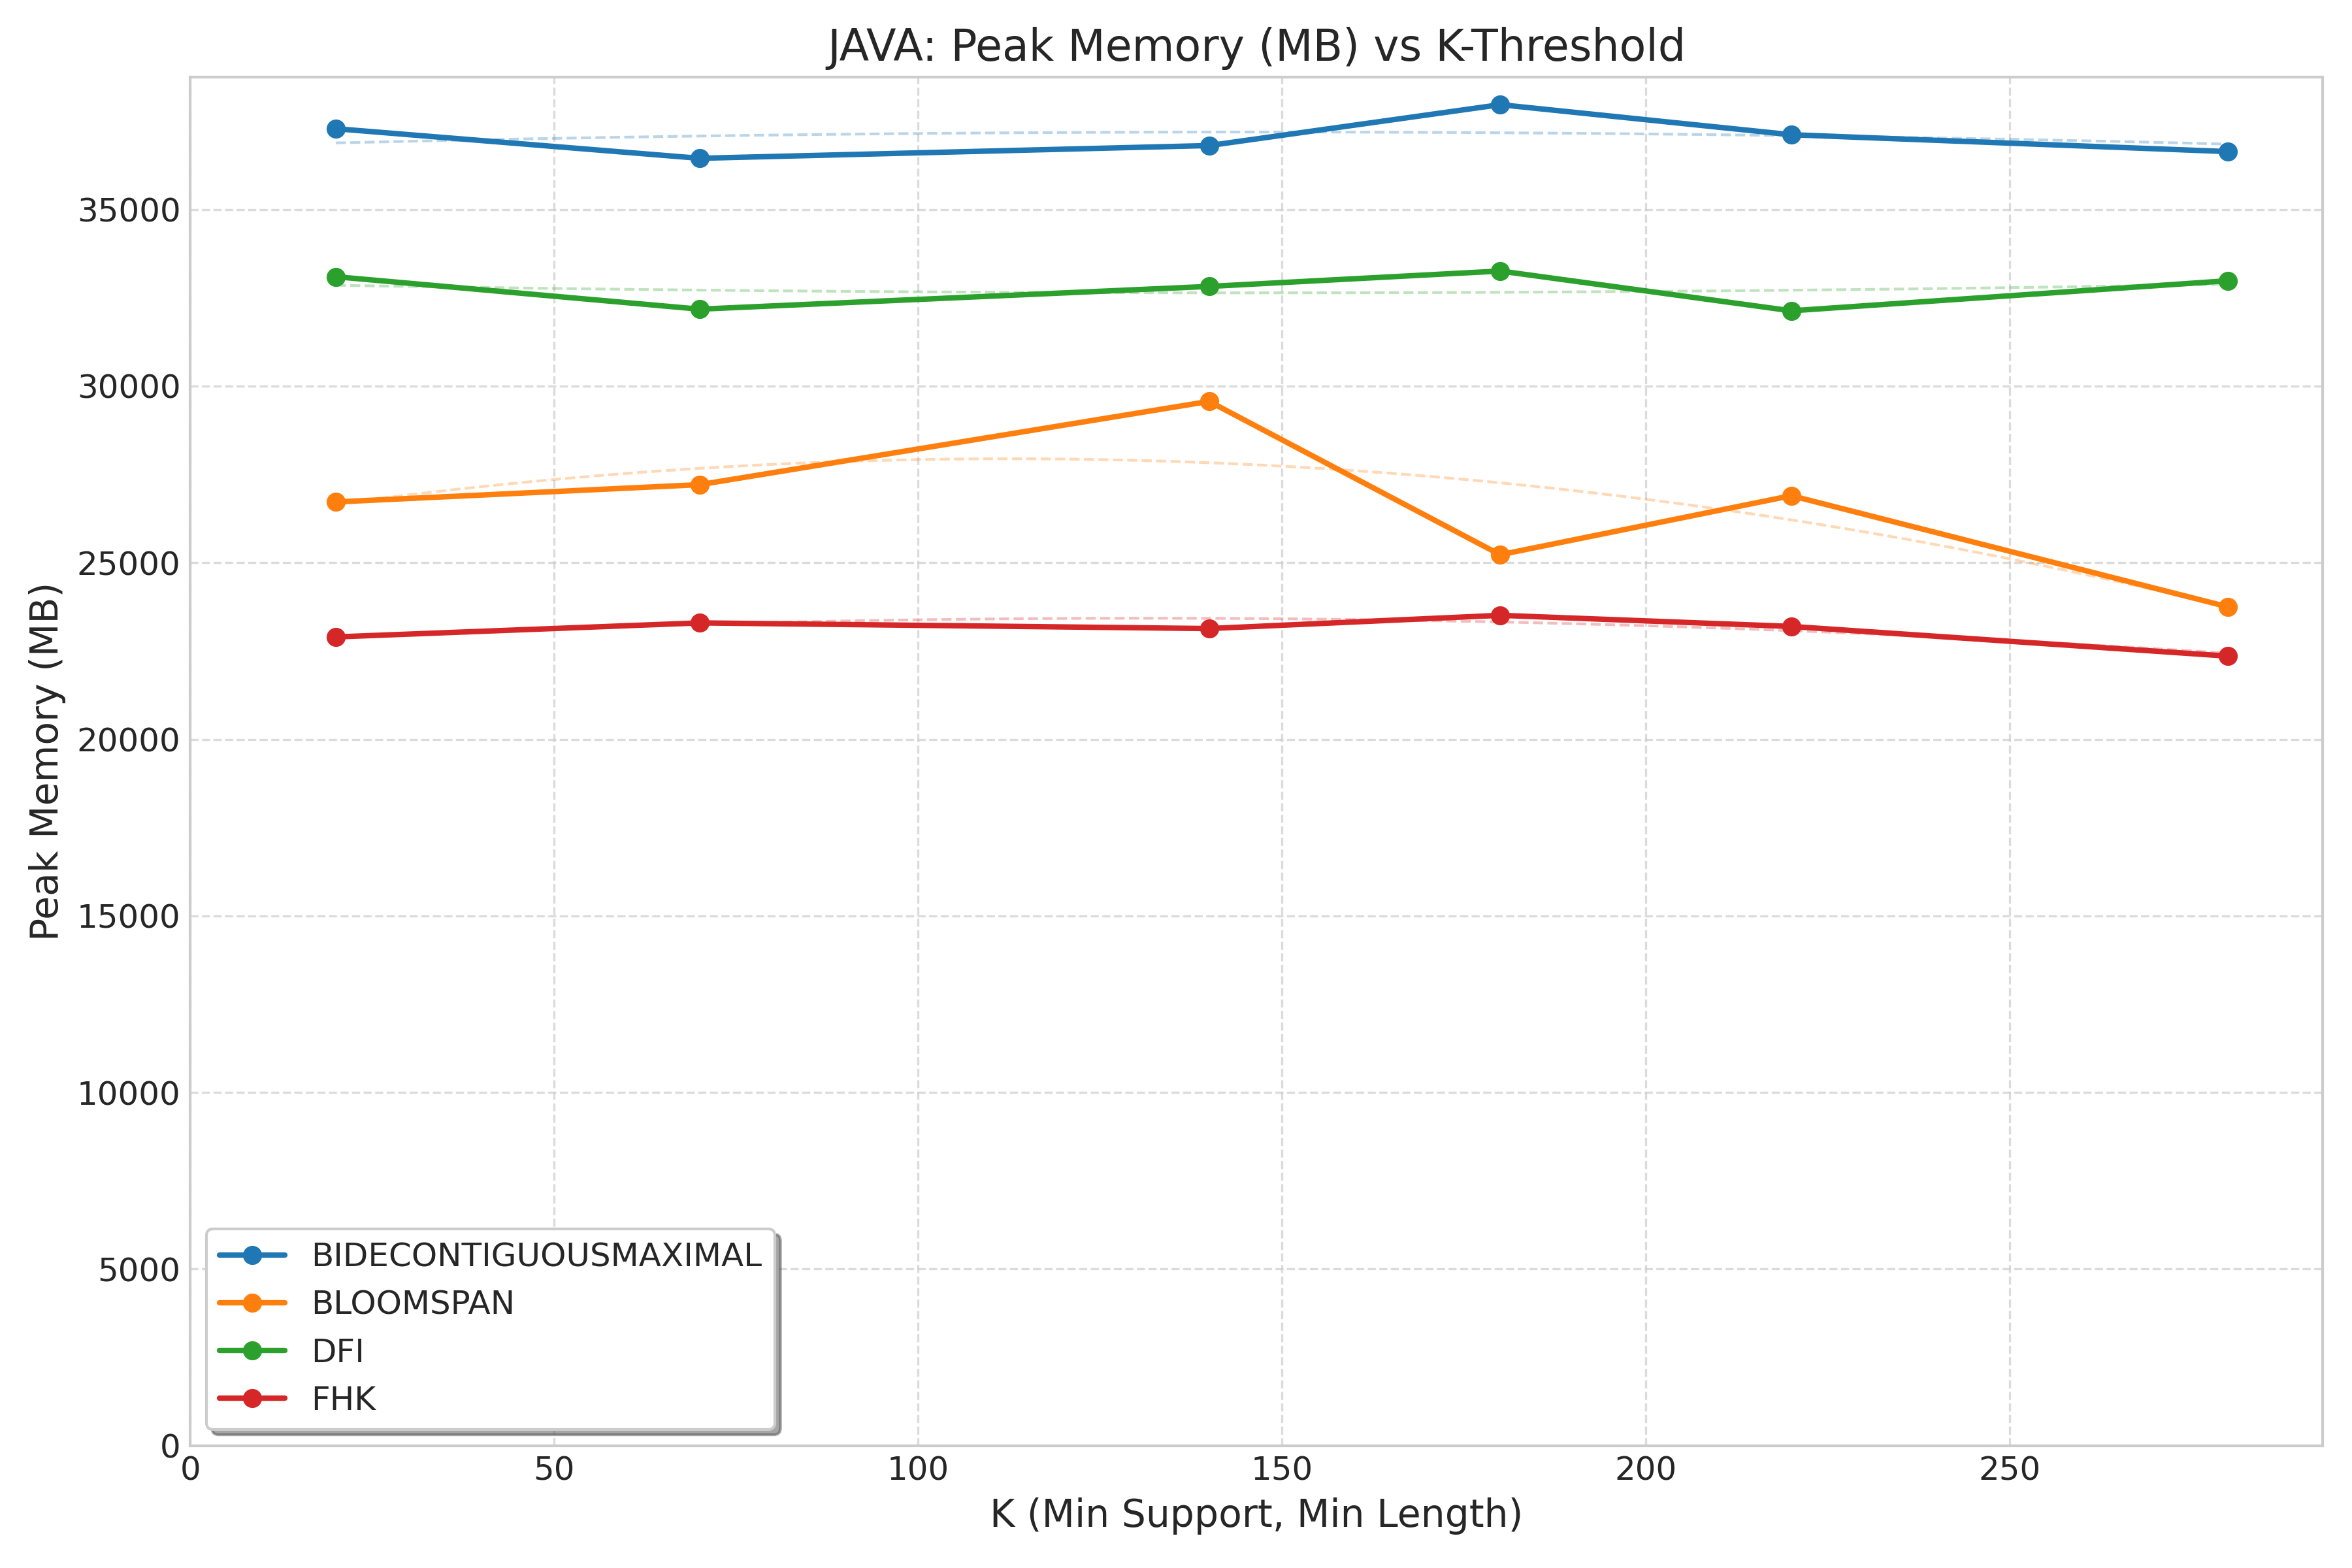
\includegraphics[width=\linewidth]{java_memory_vs_k.png}
        \end{minipage}
        \caption{Execution time (left) and peak memory (right) on Synthetic Dataset~2, $N = 15{,}000$, six runs. BIDE+ (non-maximal) and GST/SA+LCP exhaust the heap.}
        \label{fig:synth2}
    \end{figure}

    \subsection{Results: Synthetic Dataset 2 (Dense Nested Overlaps)}

    Table~\ref{tab:synth2} and Figure~\ref{fig:synth2} show results at $N = 15{,}000$ for the adversarial dataset. FHK is fastest and most memory-efficient: its LCP-interval traversal directly exploits the dense overlapping suffix structure. BloomSpan is second-fastest; its occupancy-bitmask pruning outperforms BIDE+'s per-pattern redundancy tracking despite CBF filtering losing some of its advantage when nearly every $n$-gram is frequent. BIDE+ (Contiguous, non-maximal) and GST/SA+LCP both exhaust the 40\,GB heap.


    \subsection{Results: Realistic Dataset 1 (Gutenberg-8k)}\label{sec:results-realistic}

    Table~\ref{tab:gut} shows performance on Gutenberg-8k ($\sigma = 10$, min.\ phrase length 5). SPMF-based baselines (GST/SA+LCP, BIDE+) run out of memory beyond $N = 500$. Among stringology-native algorithms, two regimes are visible: at mid-range ($N \le 1{,}000$), BloomSpan is $\approx 20\%$ faster than FHK/DFI as the CBF filter amortises; at $N \ge 3{,}000$, FHK/DFI become 10--20\% faster because the surviving MCFP set grows super-linearly under the permissive threshold ($\approx 218$k phrases at $N = 5{,}000$), making BloomSpan's output-sensitive maximality phase the bottleneck. BloomSpan runs out of memory at $N = 8{,}000$ under this operating point, while FHK and DFI complete. The MCFP sets of BloomSpan, FHK, and DFI are sorted and compared at every $N \in \{100, 250, 500, 1{,}000, 1{,}500, 3{,}000, 5{,}000\}$; all sets are identical across all measured configurations, confirming no false negatives or false positives relative to two independently implemented exact baselines. We do not claim equivalence beyond $N = 5{,}000$ where no exact baseline completes simultaneously.

    \begin{table}[!tbp]
        \caption{Performance on Gutenberg-8k ($\sigma=10$, min.\ phrase length $5$). Time in ms; memory in MB. Medians over 10 runs.}
        \begin{center}
            \resizebox{\textwidth}{!}{%
                \begin{tabular}{|c|cc|cc|cc|cc|cc|}
                    \hline
                    \textbf{N} & \multicolumn{2}{c|}{\textbf{BloomSpan}}
                    & \multicolumn{2}{c|}{\textbf{FHK}}
                    & \multicolumn{2}{c|}{\textbf{DFI}}
                    & \multicolumn{2}{c|}{\textbf{BIDE+ (Contig.)}}
                    & \multicolumn{2}{c|}{\textbf{GST/SA+LCP}} \\
                    \cline{2-11}
                    & Time & Mem & Time & Mem & Time & Mem & Time & Mem & Time & Mem \\
                    \hline
                    100   & 713          & 727   & 625          & 220    & 655          & 416    & 1{,}275    & 1{,}136  & 2{,}373    & 798 \\
                    250   & 1{,}682      & 1{,}291 & 2{,}023     & 1{,}278 & 2{,}012     & 1{,}299 & 4{,}847    & 4{,}696  & 10{,}445   & 4{,}783 \\
                    500   & 3{,}201      & 1{,}960 & 3{,}896     & 1{,}145 & 4{,}016     & 1{,}405 & 13{,}241   & 25{,}688 & 27{,}170   & 21{,}482 \\
                    1{,}000 & 6{,}608    & 4{,}483 & 8{,}425     & 1{,}875 & 8{,}313     & 2{,}158 & OOM        & OOM      & OOM        & OOM \\
                    1{,}500 & --         & --      & 12{,}714    & 2{,}602 & 12{,}752    & 2{,}517 & OOM        & OOM      & OOM        & OOM \\
                    3{,}000 & 28{,}550   & 7{,}118 & 25{,}427    & 3{,}324 & 25{,}185    & 3{,}745 & OOM        & OOM      & OOM        & OOM \\
                    5{,}000 & 141{,}023  & 5{,}416 & 117{,}228   & 5{,}155 & 111{,}864   & 5{,}179 & OOM        & OOM      & OOM        & OOM \\
                    8{,}000 & OOM        & OOM     & 2{,}214{,}653 & 9{,}828 & 1{,}461{,}332 & 9{,}819 & OOM        & OOM      & OOM        & OOM \\
                    \hline
                \end{tabular}%
            }
            \label{tab:gut}
        \end{center}
    \end{table}

    \subsection{Results: Realistic Dataset 2 (Gutenberg-BookCorpus-Cleaned)}\label{sec:results-large}

    Table~\ref{tab:real2-mining} and Figure~\ref{fig:real2} report total wall-clock time and peak heap on nine subsets (1{,}000--50{,}000 documents, $\approx 64$\,M--$3.07$\,B tokens). Each configuration used six runs (one warm-up discarded); medians with IQR are reported.  BloomSpan is 11--15$\times$ faster than FHK across every point where both complete (Table~\ref{tab:real2-mining}). The memory advantage grows with $N$: at $N = 15{,}000$, FHK uses 31.5\,GB versus BloomSpan's 15.0\,GB. DFI's $O(n \log n)$ RMQ sparse table consumes $\approx 29.4$\,GB already at $N = 3{,}000$ and fails with OOM at
    $N = 5{,}000$. FHK completes through $N = 30{,}000$ before exceeding the heap. BloomSpan completes all nine subsets including $N = 50{,}000$.

    BloomSpan's per-token mining cost on this operating point is approximately constant up to $N = 30{,}000$: measured in $\mu$s/token  for the table's mining-only values, it sits in the range $0.021$--$0.027$ across that range (a $\approx 28 \times$ increase in input size), corresponding to near-linear scaling with a log-log slope of $0.98$. At $N = 50{,}000$ the per-token cost jumps to  $0.125\,\mu$s/token as the surviving pattern set reaches     $12{,}244$ MCFPs and the output-sensitive maximality-check phase becomes visible in the mining time; log-log slope over all nine points is $1.24$. This super-linear point is nevertheless the only configuration that completes on a 3\,B-token corpus under the 40\,GB heap among all tested algorithms.

    \begin{table}[!tbp]
        \caption{BloomSpan vs.\ FHK vs.\ DFI on \texttt{Gutenberg-BookCorpus-Cleaned}
        ($\sigma = 20$, min.\ phrase length 10). Wall-clock time in seconds; peak heap memory in MB.
        Medians over five measured runs. Speedup = FHK\,/\,BloomSpan time. OOM = Out of Memory (40\,GB heap).}
        \begin{center}
            \resizebox{\textwidth}{!}{%
                \begin{tabular}{|c|cc|cc|cc|c|c|}
                    \hline
                    \textbf{N} & \multicolumn{2}{c|}{\textbf{BloomSpan}}
                    & \multicolumn{2}{c|}{\textbf{FHK}}
                    & \multicolumn{2}{c|}{\textbf{DFI}}
                    & \textbf{Speedup}
                    & \textbf{MCFPs} \\
                    \cline{2-7}
                    & Time (s) & Mem (MB) & Time (s) & Mem (MB) & Time (s) & Mem (MB) & (FHK/BS) & \\
                    \hline
                    1{,}000  &   1.73 &  5{,}095 &   19.08 &  6{,}591 &   20.17 &  9{,}138 & 11.0$\times$ &     31 \\
                    3{,}000  &   4.16 &  7{,}836 &   60.34 &  7{,}856 &   67.25 & 29{,}393 & 14.5$\times$ &    120 \\
                    5{,}000  &   6.64 &  6{,}977 &  101.33 & 11{,}238 &     OOM &      OOM & 15.3$\times$ &    217 \\
                    8{,}000  &  10.41 &  8{,}853 &  160.37 & 16{,}708 &     OOM &      OOM & 15.4$\times$ &    375 \\
                    10{,}000 &  13.59 & 12{,}044 &  199.34 & 20{,}764 &     OOM &      OOM & 14.7$\times$ &    516 \\
                    15{,}000 &  20.80 & 14{,}979 &  308.67 & 31{,}549 &     OOM &      OOM & 14.8$\times$ &  1{,}034 \\
                    20{,}000 &  27.67 & 20{,}839 &      -- &       -- &     OOM &      OOM &           -- &  1{,}964 \\
                    30{,}000 &  44.61 & 29{,}385 &  662.24 & 38{,}461 &     OOM &      OOM & 14.8$\times$ &  3{,}673 \\
                    50{,}000 & 383.27 & 38{,}873 &     OOM &      OOM &     OOM &      OOM &           -- & -- \\
                    \hline
                \end{tabular}%
            }
            \label{tab:real2-mining}
        \end{center}
    \end{table}

    \begin{figure}[!tbp]
        \begin{minipage}{0.49\textwidth}
            \centering
            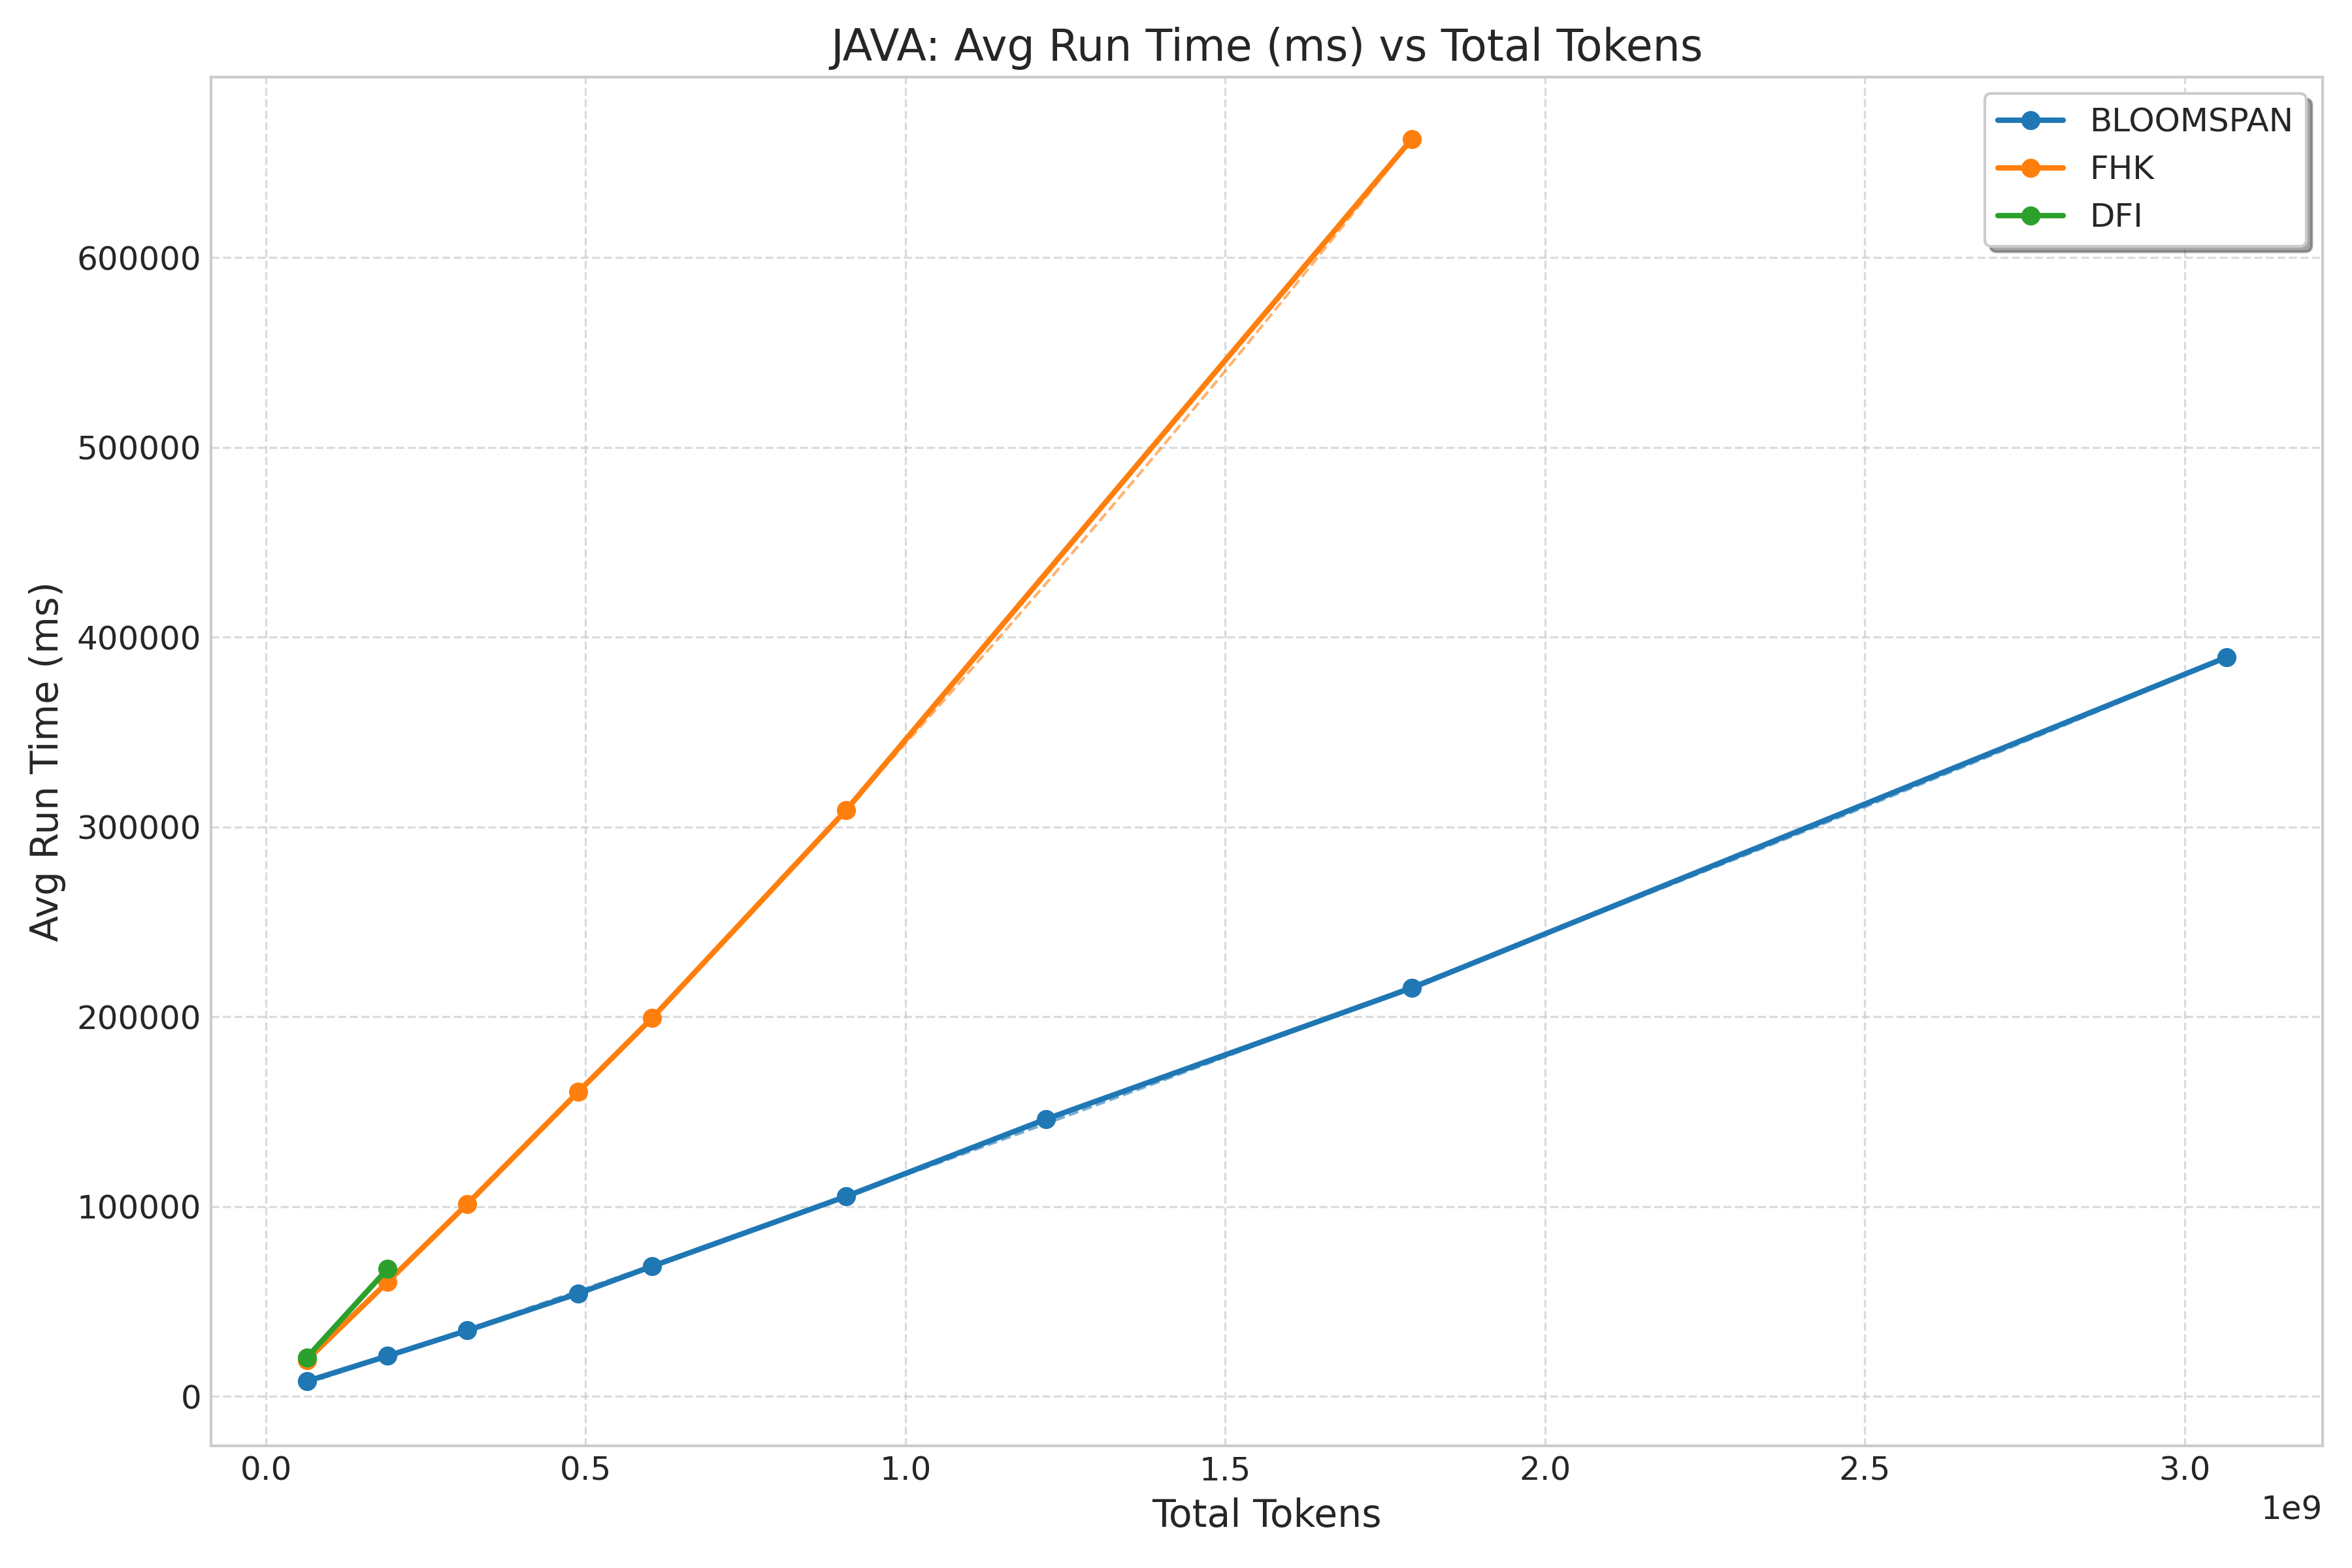
\includegraphics[width=\linewidth]{gutenberg_time.png}
        \end{minipage}
        \hfill
        \begin{minipage}{0.49\textwidth}
            \centering
            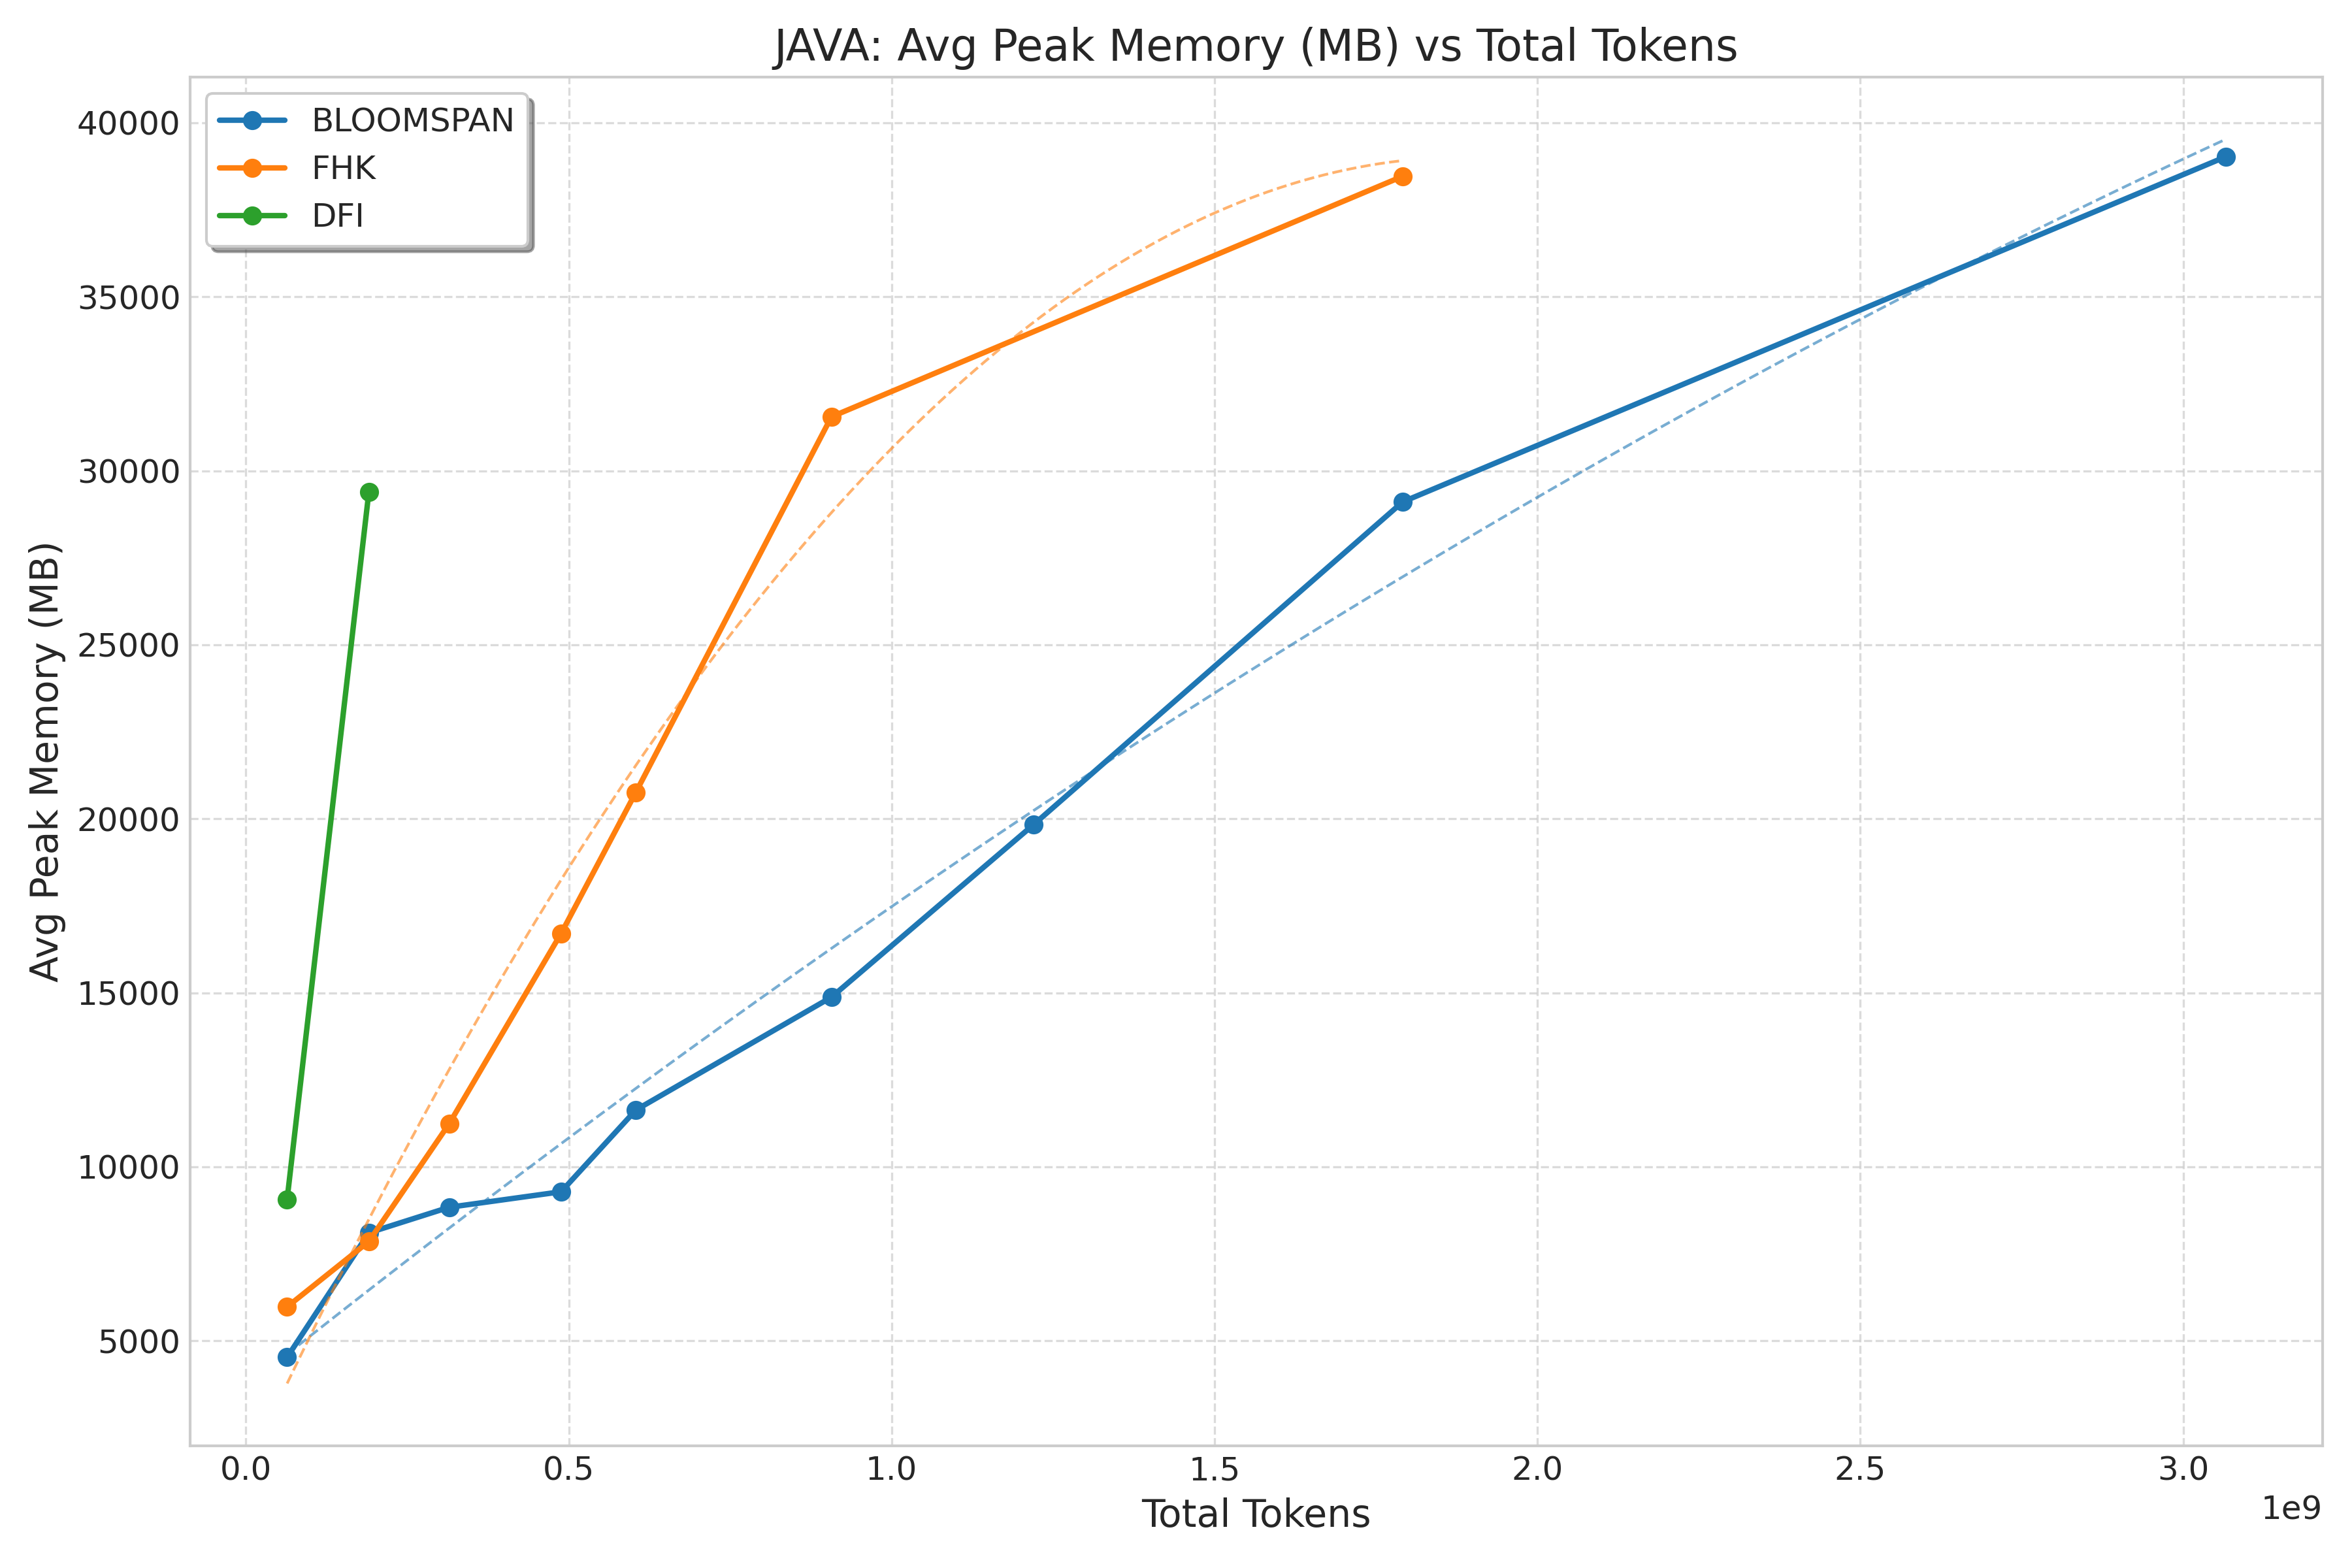
\includegraphics[width=\linewidth]{gutenberg_memory.png}
        \end{minipage}
        \caption{Wall-clock time (left) and peak heap memory (right) on \texttt{Gutenberg-BookCorpus-Cleaned} ($\sigma = 20$, min.\ phrase length 10). DFI exhausts the heap beyond $N = 3{,}000$, $tokens=190M$; FHK completes through $N = 30{,}000$, $tokens=1,7B$.}
        \label{fig:real2}
    \end{figure}

    \subsection{Topological Analysis of Datasets}

    The performance differences across datasets stem from measurable structural properties of each corpus. Let $c$ denote the number of Lempel-Ziv phrases and $n$ the total token count.

    \textbf{Synthetic Dataset 1 (Sparse Injections).} Background words are entirely unique, yielding a nearly flat frequency distribution and a maximized phrase generation ratio ($c/n \approx 0.99$, $C_{LZ} \approx 24.4$ bits/token). Under these conditions the CBF operates at peak efficiency, pruning non-repeating background noise with zero false negatives and minimal memory overhead. BloomSpan therefore scales near-linearly and decisively outruns the gap-aware miners (BIDE+, GST/SA+LCP). Among stringology-native baselines, FHK is consistently faster: its LCP-interval traversal directly enumerates maximal substrings without a separate seed-filtering pass, so BloomSpan's CBF lookup is pure overhead here. Before the crossover point, $N=12{,}000$, BloomSpan's advantage on this topology is memory. Because the background consists of entirely unique tokens, the phrase generation ratio is maximized ($c/n \approx 0.99$). In such a "flat" distribution, BloomSpan's Counting Bloom Filter (CBF) provides less pruning benefit relative to its overhead, whereas FHK’s suffix-array structures handle the lack of deep branching more natively.

    \textbf{Synthetic Dataset 2 (Dense Nested Overlaps).} The 300 heavily overlapping injections shift the topological advantage to suffix-based structures: FHK compresses identical overlapping prefixes and suffixes into a single LCP-interval traversal, neutralising the combinatorial explosion. BloomSpan's CBF-based pruning loses much of its advantage because nearly every $n$-gram in the injected pattern family is frequent; the maximality-verification phase does most of the work. Despite this, BloomSpan finishes ahead of BIDE+ (Contiguous Maximal Mode) because BIDE+'s per-pattern redundancy tracking scales poorly with deeply nested overlaps.

    \textbf{Realistic Datasets (Project Gutenberg).} Natural language provides a balanced, organic topology with a low phrase generation ratio ($c/n \approx 0.27$) and an LZ entropy rate of roughly $7.94$ bits/token. This is the domain BloomSpan is designed to exploit. The Zipfian frequency distribution~\cite{zipf1949human} typical of natural language produces a long tail of infrequent $n$-grams; the CBF prunes this tail effectively, eliminating 98\% of candidate seeds at $\sigma = 20$ (Section~\ref{sec:results-large}). The moderate compressibility also indicates that patterns are not pathologically nested, preventing the exponential memory explosion that cripples GST/SA+LCP and BIDE+ on real text and allowing BloomSpan's occupancy matrix to efficiently suppress redundancies. On Realistic Dataset 2 under a stricter operating point the output-sensitive phase stays sub-critical, and BloomSpan achieves the near-linear per-token scaling reported in Section~\ref{sec:results-large}.

    \section{Conclusion and Future Work}

    We presented BloomSpan, an algorithm for MCFP mining that combines a Counting Bloom Filter with prioritized depth-first expansion and a global occupancy bitmask, targeting natural-language corpora at strict support thresholds.

    Evaluation on four datasets reveals clear algorithm-topology trade-offs. On both synthetic datasets (sparse injections and dense nested overlaps) FHK is the fastest in wall-clock time, with BloomSpan second; on sparse injections at large $N$ BloomSpan uses the least memory among stringology-native miners. On Gutenberg-8k at the permissive threshold $\sigma = 10$, FHK/DFI are marginally faster at scale as BloomSpan's data-dependent expansion phase becomes the bottleneck. At a strict-threshold large-scale configuration (Realistic Dataset~2, $\sigma = 20$, minimum length 10, up to 3\,B tokens), BloomSpan is 11--15$\times$ faster than FHK, scales near-linearly per token up to $N = 30{,}000$ (log-log slope 0.98), and is the only evaluated algorithm completing at $N = 50{,}000$ within a 40\,GB heap. Classical gap-aware miners (BIDE+, VMSP, GST/SA+LCP) OOM at all but the smallest scales on realistic corpora.

    Future directions include near-duplicate pattern support (edit-distance tolerance), a distributed implementation with a shared CBF, and validation on non-literary domains such as genomic sequences and system event logs.

    \small
    \bibliographystyle{splncs04}
    \bibliography{literature}

\end{document}
